\documentclass{article}
\usepackage{graphicx} % Required for inserting images
\usepackage{amsthm}
\usepackage{amssymb}
\usepackage{subcaption}
\usepackage{amsmath}
\usepackage{tikz}
\usepackage{float}

\theoremstyle{definition}
\newtheorem{definition}{Definition}[section]
\newtheorem{question}{Question}[section]
\newtheorem{theorem}{Theorem}[section]
\newtheorem{lemma}{Lemma}[section]
\newtheorem{corollary}{Corollary}[section]
\newtheorem{conjecture}{Conjecture}[section]

\title{Fall 2024 Koch Curve Inversion Project}
\author{Ethan Kalika}
\date{December 2024}

\begin{document}
\maketitle
\begin{abstract}
    The goal of this research project is to find, if one exists, an algorithm for inverting the Koch curve. The problem of Koch curve inversion, is significant because its solution may give insight into the larger open problem of whether or not any bi-Lipschitz self-mapping of the plane can be factored into mappings of small distortion. This paper gives the necessary background information including a literature review covering the Carpenters Rule problem and some related problems and then details a first but unsuccessful attempt at finding an algorithm for Koch curve inversion. The shortcomings of this attempt are then used to motivate the literature review of several topics in topology. While answering the Koch curve problem remains a work in progress, this paper serves to show the current progress made in that direction.
\end{abstract}
\section{Introduction}
In the 1950's Arthur Samuel's invention of a program that could learn to play checkers and his coining of the term ``machine learning" put the concept of artificial intelligence into focus. The first machine learning programs were simple, but in time the field became very expansive. Advanced algorithms like those used for dimensionality reduction, clustering, optimization, and much more, quickly shifted the attention of scientists to data visualization schemes and realms of geometry. Then, in the 1980's Mikhail Gromov's pioneering of the field of geometric group theory, popularized contemporary geometry even more. This focus on geometry forced mathematicians to consider transformations of geometric frameworks, and, inevitably, begged questions like: ``Which types of geometric properties are preserved by which transformations?" \cite{bah2013energyawareadaptivebilipschitzembeddings}\vspace{0.5em}\\
Bi-Lipschitz mappings are the perfect tool to answer some of the questions about preservation of geometric structure during transformations because they formalize the notion of length distortion resulting from transformations from one metric space to another. Because of this, bi-Lipschitz mappings are very useful in the study of modern geometry. It was this mesh of interrelated fields like analysis, geometry, and metric spaces, that gradually generated the bi-Lipschitz mapping factorization problem. One of the first papers to touch upon this problem is Michael H. Freedmans and Zheng-Xu He's publication on factoring the logarithmic spiral and quasi-conformal mappings \cite{Freedman1988}.\vspace{0.5em}\\
The bi-Lipschitz mapping factorization problem is difficult, and one could say that there is an entire realm of mathematics dedicated just to studying Lipschitz mappings. The goal of this project is to gain insight into the bi-Lipschitz mapping factorization problem by, instead of facing it directly, focusing on a smaller related problem about inverting the Koch curve. The construction of the Koch curve and what it means to invert it will be discussed more in Sections 4. At a high level, the idea is that if there exists no continuous transformation that can invert the Koch curve, then there is a contradiction to the general statement of the bi-Lipschitz mapping factorization problem.\vspace{0.5em}\\
While this paper does not solve the Koch curve inversion problem, and is only a part of a larger project aimed at doing so, it outlines the current progress made in this direction. In Section 2 and 3, we provide background theory useful for reasoning about the Koch curve. In Section 4 we define, and prove some useful facts about the curve. Then, in Section 5 we will explore a first and unsuccessful attempt at finding an algorithm for Koch curve inversion, and finally, in Section 6 we will use the flaws of this first approach to motivate a literature review of topics in topology. The goal of this research remains figuring out how to invert the Koch curve.
\section{Basic Graph Theory, Set Theory, and Geometry}
We begin by introducing some basic graph theory because it will sometimes be useful to think of the frameworks we will be working with as graphs.
\begin{definition}
    A \textbf{graph} is an ordered pair $G = (V, E)$ where $V$ is a set of vertices and $E \subseteq \{\{x, y\}|x, y \in V$ and $x \neq y\}$.
\end{definition}
\begin{definition}
    In a graph, an \textbf{edge}, is an unordered pair of vertices.
\end{definition}
\begin{definition}
    In an edge, $\{x, y\}$, $x$ and $y$ are \textbf{endpoints}. An edge $\{x, y\}$ is said to \textbf{join} $x$ and $y$ or, to be \textbf{incident} on $x$ and $y$.
\end{definition}
\noindent While graphs are defined as sets they are most often drawn as pictures. This visualization is almost always more useful and intuitive than the set definition. Figure 1 shows an example of a graph.\vspace{0.5em}\\
\begin{figure}[h]
    \centering
    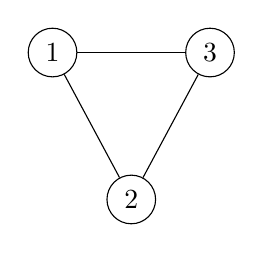
\begin{tikzpicture}
        \node[draw, circle] (1) at (0, 0) {2};
        \node[draw, circle] (2) at (-1, 1.866) {1};
        \node[draw, circle] (3) at (1, 1.866) {3};
        \draw (1) -- (2);
        \draw (2) -- (3);
        \draw (3) -- (1);
    \end{tikzpicture}
    \caption{This is a graph with three vertices and three edges. We can define this graph as follows $G = (\{1, 2, 3\}, \{\{1, 2\}, \{2, 3\}, \{3, 1\}\})$. Here the edges are $\{1, 2\}, \{2, 3\}$, and $\{3, 1\}$ while $\{1, 2, 3\}$ is just a set containing the vertices. This is the first and only time we will give the set definition of a graph, henceforth, we shall treat them mostly as geometric frameworks.}
\end{figure}
\noindent Now we give some background on the notion of convex sets, convex hulls, and norms. These are important concepts for understanding the first attempt at inverting the Koch curve presented in Section 5.
\begin{definition}
    A set, S, in a plane is called a \textbf{convex set} if each pair of points in S can be joined by a line segment lying entirely within S.
\end{definition}
\noindent Figure 2 shows a visualization of convex and non-convex sets. In Section 3, the word convex will be used to refer to curves. In the context of Section 3 it is better to think of convex as referring to the region enclosed by the curve and not the curve itself. Convex sets will be used as they are defined here in Section 5 when we will be defining convex hulls on the Koch curve.
\begin{figure}[h]
    \centering
    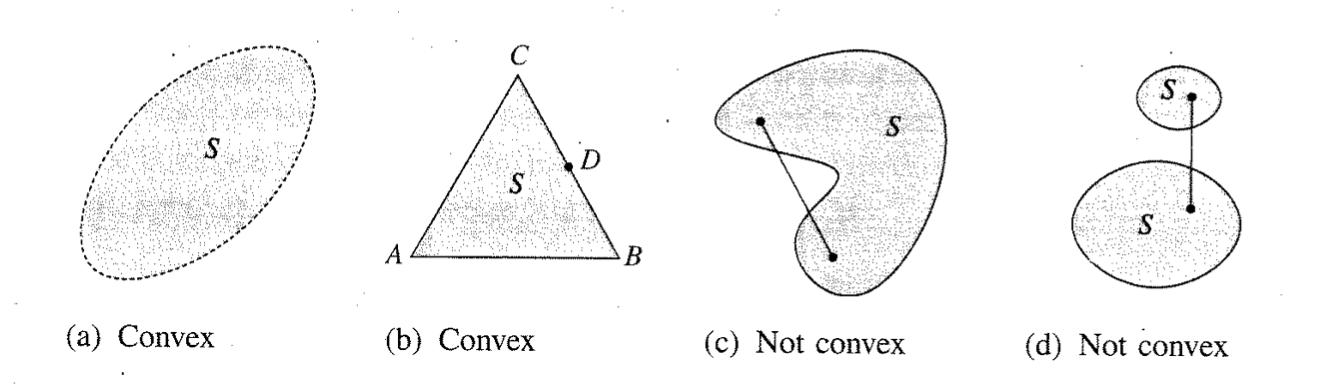
\includegraphics[width=1\textwidth]{ConvexImage.png}
    \caption{(a) and (b) are convex and (c) and (d) are not. \cite{sydsæter2005further}}
\end{figure}
\begin{definition}
    Given two vectors $\mathbf{x}$ and $\mathbf{y}$ the \textbf{convex combination} of $\mathbf{x}$ and $\mathbf{y}$ is the set $\{\lambda \mathbf{x} + (1 - \lambda)\mathbf{y}|\lambda \in [0, 1]\}$.
\end{definition}
\begin{definition}
    If S is an arbitrary set in $\mathbb{R}^n$, the \textbf{convex hull} of S is the union of all convex combinations of points in S.
\end{definition}
\noindent Figures 3 and 4 show two examples of sets and their corresponding convex hulls.
\begin{figure}[h]
    \centering
    \begin{minipage}{0.45\textwidth}
        \centering
        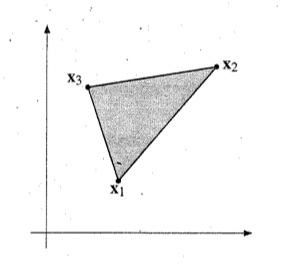
\includegraphics[height=5cm]{ConvexHull1.png}
        \caption{Here $\mathbf{x_1}$, $\mathbf{x_2}$, and $\mathbf{x_3}$ are vectors in $\mathbb{R}^2$. The line segments connecting each pair of points is the convex combination of those two points. The entire region consisting of the shaded area, the three points, and the edges between them is the convex hull of $\{\mathbf{x_1}, \mathbf{x_2}, \mathbf{x_3}\}$. \cite{sydsæter2005further}}
    \end{minipage}
    \hfill
    \begin{minipage}{0.45\textwidth}
        \centering
        \raisebox{2.2cm}{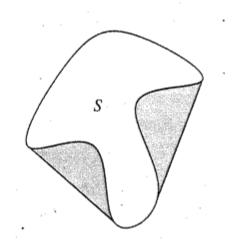
\includegraphics[height=5cm]{ConvexHull2.png}}
        \caption{Here the white region, $S$, is the set. The convex hull of $S$ includes $S$ and the shaded regions. \cite{sydsæter2005further}}
    \end{minipage}
\end{figure}
\begin{definition}
    A \textbf{norm} is a function \(||\cdot||\) satisfying, for all \(n\) dimensional vectors \(\mathbf{v}\), \(\mathbf{w}\):
    \begin{enumerate}
        \item $||\mathbf{v}|| \geq 0 \text{,} \ \text{with equality if and only if} \ \mathbf{v} = \mathbf{0}$
        \item $||\alpha\mathbf{v}|| = |\alpha| ||\mathbf{v}|| \ \text{for any scalar alpha}$
        \item $||\mathbf{v} + \mathbf{w}|| \leq ||\mathbf{v}|| + ||\mathbf{w}||$.
    \end{enumerate}
\end{definition}
\begin{definition}
    Let $\mathbf{v} \in \mathbb{R}^n$ and $v_i$ represent the $i^{th}$ coordinate of $\mathbf{v}$. For $p \geq 1$ the \textbf{p-norm} is denoted $||\mathbf{v}||_p$, and defined by
    $$||\mathbf{v}||_p = \left( \sum_{i = 1}^n|v_i|^p \right)^{1/p}.$$
\end{definition}
\noindent From this point in we will use $||\cdot||$ to represent the Euclidean norm. This will not create ambiguity because we will not have to refer to general norms.
\section{Straightening Polygonal Arcs and Convexifying Polygonal Cycles}
Straightening Polygonal Arcs and Convexifying Polygonal Cycles is a paper written by Robert Connelly, Erik D. Demaine, and G\"unter Rote. In this work, the three authors detail their solution to the Carpenter's Rule Problem and several related problems. This paper provides a framework that is critical for the rest of the discussion and serves as a motivation for the work to be done in this project. We begin by providing some important definitions leading up to the main result from this paper. This result is helpful in framing our own question about inverting the Koch curve in the beginning of Section 5. For a deeper read on related concepts refer to \cite{892131}. As mentioned previously, some of the definitions given here will describe curves as being convex. In this section, to apply the definition of convex as it was given in Section 2, it is better to think of convex as referring to the region inside a curve and not the curve itself.
\begin{definition}
    A \textbf{polygonal arc} or \textbf{open polygonal chain} is a sequence of finitely many line segments in the plane connected in a path without self-intersection.
\end{definition}
\noindent Polygonal arcs can be thought of and will in many cases be treated as graphs. The definitions presented in this section often refer to edges of polygonal arcs, as we will later see, these are the exact same edges as the ones in graphs. Similarly, the points of connection between the edges are the vertices of the graph representing the polygonal arc.
\begin{question}
    The \textbf{Carpenter's Rule Problem} asks whether a polygonal arc can be moved continuously in such a way that each edge remains a fixed length, there are no self-intersections during the motion, and at the end of the motion, the arc lies on a straight line.
\end{question}
\begin{definition}
    A \textbf{closed polygonal chain}, or, more simply, a \textbf{polygon} is a simple closed polygonal arc.
\end{definition}
\noindent In this context, simple means non-self-intersecting. Polygons can be thought of as graphs in the same sense that polygonal chains can. A related question to the Carpenter's Rule Problem is the following.
\begin{question}
    Is it possible to continuously move a polygon in a plane without creating self-intersection or changing the lengths of edges so that it ends up a convex closed curve.
\end{question}
\noindent The following is a question that is not posed in the paper, but we state it here as a possible avenue for future research.
\begin{question}
    What is the maximum number of vertices we can keep fixed while convexifying a polygon?
\end{question}
\begin{definition}
    An arc is \textbf{straightened} by a motion if at the end of the motion it lies on a straight line.
\end{definition}
\begin{definition}
    A \textbf{proper motion} is one that preserves edge length and does not cause self-intersection.
\end{definition}
\begin{definition}
    An \textbf{arc-and-cycle set} is a finite number of polygonal arcs and polygonal cycles in a plane, with none of the arcs or cycles intersecting each other or having self-intersections.
\end{definition}
\begin{definition}
    We say that an arc-and-cycle set, A, is an \textbf{outer convex configuration} if each component of A not contained inside a cycle is either straight, if it is a polygonal arc or convex, if it is a polygonal cycle.
\end{definition}
\begin{definition}
    A motion of an arc-and-cycle set is an \textbf{expansive motion} if and only if for any pair of vertices in the set, the distance between them is monotonically non-decreasing over time.
\end{definition}
\noindent Here, it is worth noting the following two facts. Firstly, if, in an expansive motion, two adjacent bars become collinear, they will remain so. Similarly, in any expansive motion once a cycle becomes convex, the cycle and any components it contains become a single rigid object.
\begin{definition}
    A \textbf{strictly expansive motion} is a motion in which the distance between two vertices connected by a bar or a set of collinear bars and between two vertices on the boundary of or interior to a common convex cycle is constant, but the distance between all other pairs of vertices monotonically strictly increases over time.
\end{definition}
\begin{definition}
    An arc-and-cycle set is \textbf{separated} if there exists a line $L$ such that $L$ is disjoint from A and at least one component of A lies on each side of $L$.
\end{definition}
\noindent The following two theorems are the main result of the paper. Both of these theorems answer an even more general question than the Carpenter's Rule Problem because they deal with arc-and-cycle sets, whereas Carpenter's rule problem asks specifically about single polygonal arcs.
\begin{theorem}
    Every arc-and-cycle set has a piecewise-differentiable proper motion to an outer-convex configuration. Moreover, the motion is strictly expansive until the arc-and-cycle set becomes separated.
\end{theorem}
\begin{theorem}
    Every arc-and-cycle set has a strictly expansive piecewise differentiable proper motion to an outer convex configuration.
\end{theorem}
\noindent Now that we have stated the main results of the paper, the remaining part of this section will present the theory that motivates the attempt to straighten the Koch curve presented in Section 5.
\begin{definition}
    A \textbf{bar framework} or \textbf{linkage framework}, denoted $G(\mathbf{p})$ is a finite graph $G = (V, E)$ without loops or multiple edges, together with a corresponding configuration $\mathbf{p} = (\mathbf{p_1}, \ldots, \mathbf{p_n})$ of $n$ distinct points in the plane where $\mathbf{p_i}$ corresponds to vertex $i \in V$. For convenience, we assume $V = \{1, \ldots, n\}$.
\end{definition}
\begin{definition}
    A \textbf{Flex} or \textbf{motion of G(p)} is a set of continuous functions $\mathbf{p}(t) = (p_1(t), \ldots, p_n(t))$, defined on $0 \leq t \leq 1$, such that $\mathbf{p}(0) = \mathbf{p}$ and the Euclidean distance $||\mathbf{p_i}(t) - \mathbf{p_j}(t)||$ is constant for each $\{i, j\} \in E$.
\end{definition}
\begin{lemma}
    Suppose the closed triangle $\mathbf{p_1p_2p_3}$ and the points $\mathbf{c}$ and $\mathbf{q_3}$ are contained in a plane and let $\mathbf{c}$ be in $\mathbf{p_1p_2p_3}$. If $||\mathbf{q_3} - \mathbf{p_2}|| \geq ||\mathbf{p_3} - \mathbf{p_2}||$ and $||\mathbf{q_3} - \mathbf{p_1}|| \geq ||\mathbf{p_3} - \mathbf{p_1}||$ then $||\mathbf{q_3} - \mathbf{c}|| \geq ||\mathbf{p_3} - \mathbf{c}||$ with equality only if $||\mathbf{q_3} - \mathbf{p_2}|| = ||\mathbf{p_3} - \mathbf{p_2}||$ and $||\mathbf{q_3} - \mathbf{p_1}|| = ||\mathbf{p_3} - \mathbf{p_1}||$.
\end{lemma}
\noindent For proof of Lemma 3.1 refer to \cite{892131}. Figure 5 provides a visualization of lemma 3.1.
\begin{figure}[h]
    \centering
    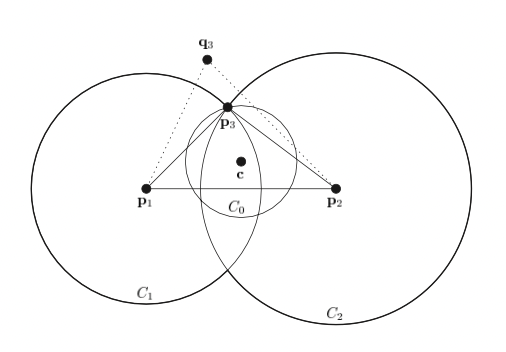
\includegraphics[width=0.8\textwidth]{Lemma1Image.png}
    \caption{Depiction of Lemma 3.1. \cite{892131}}
\end{figure}
\begin{corollary}
    Any expansive motion of an arc-and-cycle set only increases the distance between two points on the arc-and-cycle set (either a vertex or on a bar). In particular, there can be no self-intersections.
\end{corollary}
\noindent For proof of Corollary 3.1 refer to \cite{892131}.
\section{The Koch Curve}
There are several ways to define the Koch curve, here we will use a recursive process to define it. This recursive process will create a sequence of arc-and-cycle sets, the limit of this sequence being the Koch curve.\vspace{0.5em}\\
The first iteration of the process is the arc-and-cycle set consisting of single bar, as shown in Figure 6. The second iteration is the arc-and-cycle set consisting of four bars connected as shown in Figure 7.\vspace{0.5em}\\
\begin{figure}[H]
    \centering
    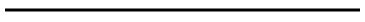
\includegraphics[width=0.5\textwidth]{Koch1.png}
    \caption{This is the first iteration of the Koch curve.}
\end{figure}
\begin{figure}[h]
    \centering
    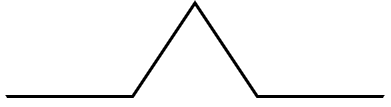
\includegraphics[width=0.5\textwidth]{Koch2.png}
    \caption{This is the second iteration of the Koch curve. Each bar in this bar framework must be between $\frac{1}{2}$ and $\frac{1}{4}$ of the length of the bar in the first iteration.}
\end{figure}
\noindent From the third iteration onward every iteration is constructed by replacing every bar in the one before it with the arc-and-cycle set form Figure 7. Figure 8 shows the third iteration, which is the result of replacing every bar in second iteration with a scaled version of the curve in Figure 7.\vspace{0.5em}\\
\begin{figure}[h]
    \centering
    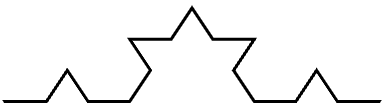
\includegraphics[width=0.5\textwidth]{Koch3.png}
    \caption{This is the third iteration of the Koch curve. It is visible how it can be derived from the second one by replacing every bar with a copy of Figure 7.}
\end{figure}
\noindent We will need to make reference to particular vertices in these arc-and-cycle sets so it is implied that each iteration can also be represented by the bar framework corresponding to the arc-and-cycle set for that iteration. This way, there is a set in which all vertices in the iteration are defined. In the bar framework for a particular iteration the vertices will be the set of points containing the endpoints of the curve and the points of connection between the bars.\vspace{0.5em}\\
The curve appearing at the limit of this iterative process is the Koch curve. Note that a bar framework must be a finite graph so the limit of this iterative process cannot be an arc-and-cycle set or a bar framework. The notion of arc-and-cycle sets is only applicable when we are working with finite iterations of the Koch curve, the Koch curve itself will be studied mainly as a curve. Figure 9 shows an arc-and-cycle set resembling the Koch curve.\vspace{0.5em}\\
\begin{figure}[h]
    \centering
    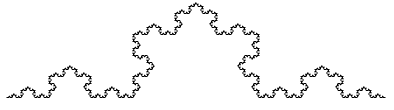
\includegraphics[width=\textwidth]{Koch6.png}
    \caption{In reality, the Koch curve cannot be depicted because it is an infinitely complex shape. What is depicted here is the $6^{\text{th}}$ iteration if the Koch curve. After this iteration the details become so fine that they would not add anything to the depiction so we use an image of the $6^{\text{th}}$ iteration to show what the actual curve may look like.}
\end{figure}
\section{An Attempt at Straightening the Koch Curve}
In this section we look at an unsuccessful attempt to unfold the Koch curve and explain why this approach does not work. After this, we use the shortcomings of the approach to motivate the next section about topology.
\begin{theorem}
    The Koch curve has a countably infinite amount of vertices.
\end{theorem}
\begin{proof}
    Each finite iteration of the curve has a finite set of vertices, and the set of vertices in the Koch curve is the union of all of these sets. Hence, the set of vertices in the Koch curve is a countably infinite union of countable sets and so must be countable.
\end{proof}
\noindent Now lets try to straighten the Koch curve. Taking inspiration from Connelly et al. and their statement in Theorem 3.1, we pose the following 2 questions.
\begin{question}
    Is there a proper motion that straightens the Koch curve? If this motion exists, then how can it be defined?
\end{question}
\noindent If we can find a proper motion that straightens the Koch curve, then inverting the curve will be a trivial matter. We propose the following method, in Conjecture 5.1, the idea of which is to simply unfold the Koch curve. We split the vertices of the Koch curve into two sets, one set containing the straightened vertices and the other the vertices yet to be straightened. We rotate the straightened tail of the curve to be in line with the first bar which is not yet straightened and continue this process all the way down the curve. Figure 10 shows this method being applied to the second iteration of the Koch curve.
\begin{conjecture}
    The following method can be used to straighten the Koch curve:
    \begin{enumerate}
        \item Choose an endpoint of the Koch curve, let the bar incident on the endpoint be the pivot bar and the other vertex intersected by the pivot bar be the pivot vertex. Also let $S$ be a set containing the chosen endpoint.
        \item Rotate all vertices in $S$ about the pivot vertex until the pivot bar is collinear with the other bar incident on the pivot vertex.
        \item Add the pivot vertex to $S$ and let the other bar incident on the pivot vertex be the new pivot bar and let the other vertex intersected by the new pivot bar be the new pivot vertex.
        \item If the pivot vertex is not an endpoint of the curve return to step 2.
    \end{enumerate}
\end{conjecture}
\noindent Before applying this method to the Koch curve, lets see how it works when applied to the finite iterations. We will see very soon, that even for the finite iterations, this approach does not work well.\vspace{0.5em}\\
\begin{figure}[H]
    \centering
    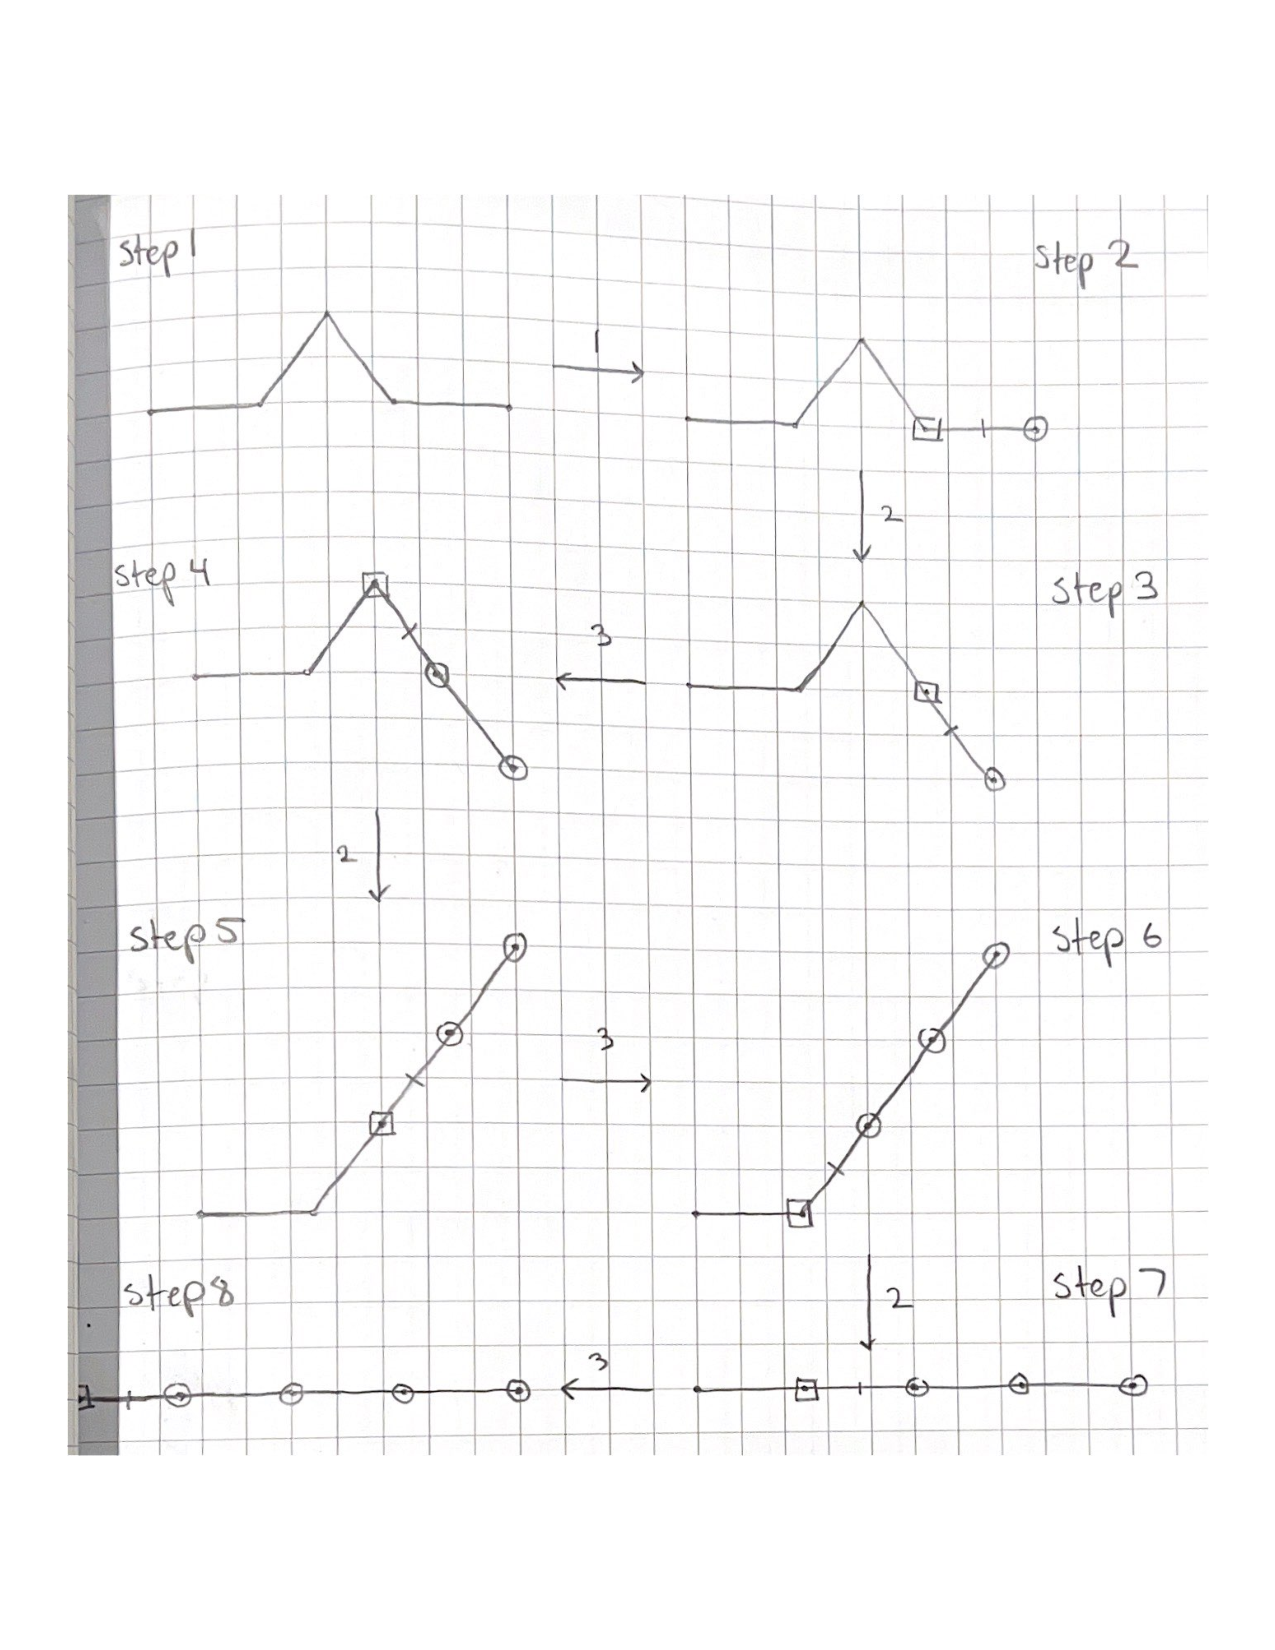
\includegraphics[width=0.8\textwidth]{KochUnfoldingMethod.pdf}
    \caption{Each step of the method application is labeled, in this case it took 8 steps to unfold the Koch curve. The arrows point in the direction of progression of the method and the number next to each arrow indicates the part of the method used to get to that step from the previous one. The encircled vertices are in the set $S$ and the boxed vertex is the pivot vertex. The bar with the dash through it is the pivot bar. The method terminated at step 8 because the pivot vertex became an endpoint of the curve.}
\end{figure}
\noindent Ideally, we would want the method in Conjecture 5.1 to be a proper motion on the finite iterations of the Koch curve. In their work, Connelly et al. showed that a motion is proper, by proving the even stronger condition, that it is strictly expansive. This is the purpose of Lemma 3.1 and Corollary 3.1. However, Conjecture 5.1 does not produce a strictly expansive motion on finite iterations of the Koch curve. This follows immediately from referring to Figure 14 and substituting the parameters $l_1 = l_2 = 5$ and $\theta = arccos(\frac{3}{5})$. Observe that with these parameter values $\mathbf{x_1}$ and $\mathbf{x_3}$ are closer in Figure 13 than in Figure 11, meaning that the motion brought them closer together and therefore is not strictly expansive.
\begin{figure}[H]
    \centering
    \begin{minipage}{0.45\textwidth}
        \centering
        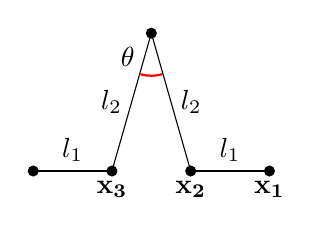
\begin{tikzpicture}
            \fill (-1, 0) circle (2pt);
            \fill (0, 0) circle (2pt) node[below] {$\mathbf{x_3}$};
            \fill (0.5, 1.75) circle (2pt);
            \fill (1, 0) circle (2pt) node[below] {$\mathbf{x_2}$};
            \fill (2, 0) circle (2pt) node[below] {$\mathbf{x_1}$};
            \draw (-1, 0) -- (0, 0) node[midway, above] {$l_1$};
            \draw (0, 0) -- (0.5, 1.75) node[midway, left] {$l_2$};
            \draw (0.5, 1.75) -- (1, 0) node[midway, right] {$l_2$};
            \draw (1, 0) -- (2, 0) node[midway, above] {$l_1$};
            \draw[red, thick] (0.363, 1.229) arc[start angle=-105.945, end angle=-74.055, radius=0.5cm];
            \node at (0.2, 1.45) {$\theta$};
        \end{tikzpicture}
        \caption{Second iteration of the Koch curve with important parameters labeled.}
    \end{minipage}
    \hfill
    \begin{minipage}{0.45\textwidth}
        \centering
        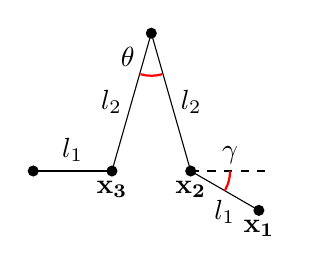
\begin{tikzpicture}
            \fill (-1, 0) circle (2pt);
            \fill (0, 0) circle (2pt) node[below] {$\mathbf{x_3}$};
            \fill (0.5, 1.75) circle (2pt);
            \fill (1, 0) circle (2pt) node[below] {$\mathbf{x_2}$};
            \fill (1.866, -0.5) circle (2pt) node[below] {$\mathbf{x_1}$};
            \draw (-1, 0) -- (0, 0) node[midway, above] {$l_1$};
            \draw (0, 0) -- (0.5, 1.75) node[midway, left] {$l_2$};
            \draw (0.5, 1.75) -- (1, 0) node[midway, right] {$l_2$};
            \draw (1, 0) -- (1.866, -0.5) node[midway, below] {$l_1$};
            \draw[dashed] (1, 0) -- (2, 0);
            \draw[red, thick] (1.433, -0.25) arc[start angle=-30, end angle=0, radius=0.5cm];
            \node at (1.5, 0.2) {$\gamma$};
            \draw[red, thick] (0.363, 1.229) arc[start angle=-105.945, end angle=-74.055, radius=0.5cm];
            \node at (0.2, 1.45) {$\theta$};
        \end{tikzpicture}
        \caption{The second iteration of the Koch curve after its right most bar has been rotated and angle of $\gamma$, this is an intermediate step of the procedure in Conjecture 5.1. This is a more general case of Figure 13.}
        \hfill
    \end{minipage}
    \begin{minipage}{0.45\textwidth}
        \centering
        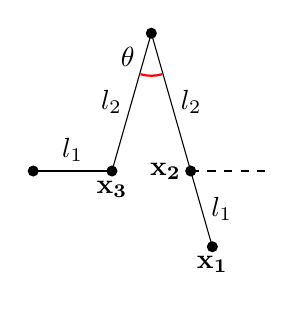
\begin{tikzpicture}
            \fill (-1, 0) circle (2pt);
            \fill (0, 0) circle (2pt) node[below] {$\mathbf{x_3}$};
            \fill (0.5, 1.75) circle (2pt);
            \fill (1, 0) circle (2pt) node[left] {$\mathbf{x_2}$};
            \fill (1.275, -0.962) circle (2pt) node[below] {$\mathbf{x_1}$};
            \draw (-1, 0) -- (0, 0) node[midway, above] {$l_1$};
            \draw (0, 0) -- (0.5, 1.75) node[midway, left] {$l_2$};
            \draw (0.5, 1.75) -- (1, 0) node[midway, right] {$l_2$};
            \draw (1, 0) -- (1.275, -0.962) node[midway, right] {$l_1$};
            \draw[dashed] (1, 0) -- (2, 0);
            \draw[red, thick] (0.363, 1.229) arc[start angle=-105.945, end angle=-74.055, radius=0.5cm];
            \node at (0.2, 1.45) {$\theta$};
        \end{tikzpicture}
        \caption{The second iteration of the Koch curve after an iteration of the method was applied to it, that is, after steps 1, 2, and 3 were applied once.}
        \hfill
    \end{minipage}
    \caption{$l_1$ and $l_2$ are lengths of bars, $\theta$ is the measure of the angle at the peak of the curve, and $\mathbf{x_1}$, $\mathbf{x_2}$, and $\mathbf{x_3}$ are the names of the vertices. Note the names of the vertices are bold because these vertices are also represented as vectors.}
\end{figure}
\noindent We can try to be clever and look at the diagram in the $l_1$ distance metric. Doing so, we can prove the following lemma, but, as we will see, even this is not to be strong enough.
\begin{lemma}
    For $\gamma \in (0, \frac{\pi}{2})$ all vertices Figure 12, are at least as far apart as they were in Figure 11 when distance is measured in the $l_1$ distance metric.
\end{lemma}
\begin{proof}
    First, lets show that $\mathbf{x_1}$ and $\mathbf{x_2}$ are farther (in the $l_1$ distance metric) in Figure 12 than in Figure 11 for any $\gamma \in (0, \frac{\pi}{2})$. In Figure 11, $||\mathbf{x_1} - \mathbf{x_2}||_1 = l_1$ and in Figure 12, $||\mathbf{x_1} - \mathbf{x_2}||_1 = l_1cos(\gamma) + l_1sin(\gamma)$. Then it is clear that for $\gamma \in (0, \frac{\pi}{2})$, this distance is greater in Figure 12.\vspace{0.5em}\\
    For any vertex, $\mathbf{v} \neq \mathbf{x_1}$, $||\mathbf{x_2} - \mathbf{v}||_1$ remains constant as $\gamma$ varies and $||\mathbf{x_1} - \mathbf{v}||_1$ = $||\mathbf{x_1} - \mathbf{x_2}||_1 + ||\mathbf{x_2} - \mathbf{v}||_1$. Then $||\mathbf{x_1} - \mathbf{v}||_1$ is greater in Figure 12 than in Figure 11.
\end{proof}
\noindent Lemma 5.1 is not strong enough to prove that the procedure in Conjecture 5.1 is a proper motion for 2 reasons. Firstly, because it shows that there are pairs of nonadjacent vertices such that the distance between them is constant, but for a motion to be strictly expansive, all nonadjacent vertices have to be monotonically strictly getting farther from one another. Secondly, Lemma 5.1 is not strong enough because it only considers the initial and terminal positions of each vertex, in order to be strictly expansive the vertices must be getting farther at each instance within the motion.\vspace{0.5em}\\
There is however, a way to show that the motion in Conjecture 5.1 is proper when applied to Figure 11. That is, we can loosen the conditions we are trying to prove, and instead of showing that Conjecture 5.1 produces a strictly expansive motion, we can show that it produces a proper motion directly. We do this by drawing a vertical line, $L$, at the pivot vertex, as shown in Figure 15. Although we do not show this rigorously, one can see that there is no way that the tail of straightened bars can cross $L$ to intersect any other part of the curve. Hence, there can never be self-intersections. Figure 15 illustrates the following lemma.
\begin{lemma}
    The method in Conjecture 5.1 produces a proper motion when applied to the arc-and-cycle set in Figure 11.
\end{lemma}
\begin{figure}[h]
    \centering
    \begin{minipage}{0.49\textwidth}
        \centering
        \begin{tikzpicture}
            \fill (-1, 0) circle (2pt);
            \fill (0, 0) circle (2pt);
            \fill (0.5, 1.75) circle (2pt);
            \fill (1, 0) circle (2pt);
            \fill (2, 0) circle (2pt);
            \draw (-1, 0) -- (0, 0);
            \draw (0, 0) -- (0.5, 1.75);
            \draw (0.5, 1.75) -- (1, 0);
            \draw (1, 0) -- (2, 0);
            \draw (1, -0.5) -- (1, 2.25) node[right] {$L$};
        \end{tikzpicture}%\vspace{0.5cm}
    \end{minipage}
    \hfill
    \begin{minipage}{0.49\textwidth}
        \centering
        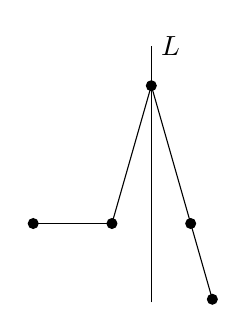
\begin{tikzpicture}
            \fill (-1, 0) circle (2pt);
            \fill (0, 0) circle (2pt);
            \fill (0.5, 1.75) circle (2pt);
            \fill (1, 0) circle (2pt);
            \fill (1.275, -0.962) circle (2pt);
            \draw (-1, 0) -- (0, 0);
            \draw (0, 0) -- (0.5, 1.75);
            \draw (0.5, 1.75) -- (1.275, -0.962);
            \draw (0.5, -1) -- (0.5, 2.25) node[right] {$L$};
        \end{tikzpicture}
    \end{minipage}
    \caption{It is visible that the tail of straightened bars can never cross a vertical line drawn at the pivot vertex as a consequence of any of the steps in Conjecture 5.1.}
\end{figure}
Even Lemma 5.1 however, is not strong enough to prove Conjecture 5.1. Figure 16 demonstrates how, for higher iterations of the Koch curve, Conjecture 5.1 can still cause self intersection.
\begin{figure}[H]
    \centering
    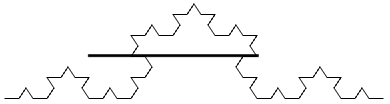
\includegraphics[width=0.75\textwidth]{KochMethodCounterexample.png}
    \caption{This is the fourth iteration of the Koch curve. The bold line indicates where the tail of straightened bars would lie when unfolding a specific bar on the right side of the curve. This tail would visibly intersect other parts of the curve causing a self-intersection.}
\end{figure}
\noindent This proves that the method in Conjecture 5.1 causes self-intersections and hence does not produce a proper motion on the Koch curve. We propose the following modifications to the method in Conjecture 5.2 to avoid self-intersections. The idea here is to just stop rotating the straightened tail of bars if it gets too close to other parts of the curve. If this does happen, then we move on without straightening a particular vertex and come back to it later once the rest of the curve has been straightened.
\begin{conjecture}
    The following method can be used to straighten the Koch curve:
    \begin{enumerate}
        \item Choose an endpoint of the Koch curve, let the bar incident on the endpoint be the pivot bar and the other vertex intersected by the pivot bar be the pivot vertex. Also, let $S$ be a set containing the chosen endpoint and $C$ be the convex hull of all the vertices in not in $S$.
        \item Rotate all vertices in $S$ about the pivot vertex until the pivot bar is collinear with the other bar incident on the pivot vertex or until a bar between a pair of vertices in $S$ gets sufficiently close to $C$.
        \item Add the pivot vertex to $S$, let the other bar incident on the pivot vertex be the new pivot bar, let the other vertex intersected by the new pivot bar be the new pivot vertex, and change C to be the convex hull of all the vertices not in $S$.
        \item If the pivot vertex is not an endpoint of the curve return to step 2.
        \item If not all the vertices on the curve are collinear then remove all vertices from $S$ and return to step 1.
    \end{enumerate}
\end{conjecture}
\noindent Conjecture 5.2 avoids self-intersection because it will simply stop rotating the straightened tail if it is about to touch any other part of the Curve. Figure 17 shows how this method would avoid the self-intersection that occurred with the method in Conjecture 5.1.\vspace{0.5em}\\
\begin{figure}[h]
    \centering
    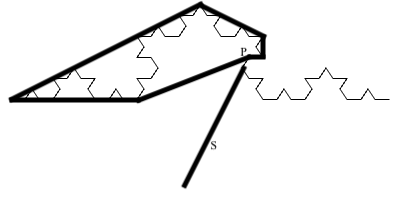
\includegraphics[width=0.8\textwidth]{NewMethodImage.png}
    \caption{P is the pivot vertex, S denotes the tail of straightened vertices, and the closed bold curve is the convex hull of all the vertices not in S. It is visible that S will hit the convex hull before becoming collinear with the non-pivot bar intersecting pivot vertex. This means the method will just change the pivot vertex and pivot bar to be the next vertex and bar in the curve and continue on, having left the angle created in the step shown. When the method reaches step 5, it will restart again from one of the endpoints and fix the angle in this figure after cycling around to it again.}
\end{figure}
\noindent Proving Conjecture 5.2 however, would still not solve the Koch curve inversion problem. The procedure outlined in Conjecture 5.2 only straightens the curve one vertex at a time. However, the Koch curve has an infinite amount of vertices, so Conjecture 5.2 would require an infinite amount of time to straighten the Koch curve. This is why the approach of simply, ``unfolding" the Koch curve does not work. To straighten the Koch curve in finite time, each step of our proposed algorithm will have to move an infinite amount of vertices. Studying such transformations requires topics in like Topology and Homotopy.
\section{Survey of Topics in Topology}
Rotating a rigid bar about a fixed point is one thing, but continuously moving infinitely many points on a fractal without causing self-intersection is an entirely different story. To do this we will need more advanced topics in geometry and Topology is a great place to start. The theory provided here is meant to just be a brief overview of concepts that may be useful for the rest of this project. For a deeper reading on these and related conceps refer to \cite{munkres2000topology}.
\begin{definition}
    A \textbf{topology} on a set $X$ is a collection $\tau$ of subsets of $X$ having the following properties:
    \begin{enumerate}
        \item $\emptyset$ and $X$ are in $\tau$
        \item The union of any subcollection of $\tau$ is in $\tau$
        \item The intersection of a finite subcollection of $\tau$ is in $\tau$
    \end{enumerate}
    A set $X$ for which a topology $\tau$ has been specified is called a \textbf{topological space}.
\end{definition}
\begin{definition}
    If $X$ is a topological space with topology $\tau$, we say a subset $U$ of $X$ is an \textbf{open set} if $U$ belongs to the collection $\tau$.
\end{definition}
\begin{definition}
    If $X$ is a set, a \textbf{basis} for the topology on $X$ is a collection $\beta$ of subsets of $X$ (called \textbf{basis elements}) such that
    \begin{enumerate}
        \item For each $x$ in $X$, there is at least one basis element $B$ containing $x$.
        \item If $x$ belongs to the intersection of two basis elements $B_1$ and $B_2$, then there is a basis element $B_3$ containing $x$ such that $B_3 \subset B_1 \cap B_2$
    \end{enumerate}
    If $\beta$ satisfies these two conditions, then we define the \textbf{topology $\tau$ generated by $\beta$} as follows: A subset $U$ of $X$ is said to be open in $X$ (that is, to be an element of $\tau$) if for each $x$ in $U$, there is a basis element $B$ in $\beta$ such that $x$ is in $B$ and $B \subset U$
\end{definition}
\begin{definition}
    Let $X$ be a topological space with the topology $\tau$. If $Y$ is a subset of $X$ the collection $\tau_Y = \{Y \cap U | U \in \tau\}$ is a topology on $Y$, called the \textbf{subspace topology}. With this topology, $Y$ is called a \textbf{subspace} of $X$; its open sets consist of all intersections of open sets $X$ with $Y$.
\end{definition}
\begin{definition}
    A subset, $A$, of a topological space $X$, is said to be \textbf{closed} if the set $X - A$ is open.
\end{definition}
\begin{definition}
    $U$ is a \textbf{neighborhood} of $x$ if $U$ is an open set containing $x$.
\end{definition}
\begin{definition}
    A topological space $X$ is called a \textbf{Hausdorff space} if for each pair $x_1, x_2$ of distinct points of $X$, there exist neighborhoods $U_1$ and $U_2$ of $x_1$ and $x_2$, respectively that are disjoint.
\end{definition}
\begin{definition}
    Let $X$ and $Y$ be topological spaces. A function $f: X \rightarrow Y$ is said to be \textbf{continuous} if for each subset $V$ of $Y$, the set $f^{-1}(V)$ is an open subset of $X$.
\end{definition}
\begin{theorem}[Rules for Constructing Continuous Functions]
    Let $X$, $Y$, and $Z$ be topological subspaces
    \begin{enumerate}
        \item(Constant Function) If $f: X \rightarrow Y$ maps all of $X$ into the single point $y_0$ of $Y$, then $f$ is continuous.
        \item(Inclusion) If $A$ is a subsequence of $X$, then inclusion function $j: A \rightarrow X$ is continuous.
        \item(Composites) If $f: X \rightarrow Y$ and $g: Y \rightarrow Z$ are continuous, then the map $g \circ f: X \rightarrow Z$ is continuous.
        \item(Restricting the domain) If $f: X \rightarrow Y$ is continuous, and if $A$ is a subspace of $X$, then the restricted function $f|A \rightarrow Y$ is continuous.
        \item(Restricting or expanding the range) Let $f: X \rightarrow Y$ be continuous. If $Z$ is a subspace of Y containing the image set $f(X)$, then the function $g: X \rightarrow Z$ obtained by restricting the range of $f$ is continuous. If $Z$ is a space having $Y$ as a subspace, then the function $h: X \rightarrow Z$ obtained by expanding the range of $f$ is continuous.
        \item(Local formulation of continuity) The map $f: X \rightarrow Y$ is continuous if $X$ can be written as the union of open sets $U_{\alpha}$ such that $f|U_{\alpha}$ is continuous for each $\alpha$.
    \end{enumerate}
\end{theorem}
\begin{theorem}[The Pasting Lemma]
    Let $X = A \cup B$, where $A$ and $B$ are closed in $X$. Let $f: A \rightarrow Y$ and $g: B \rightarrow Y$ be continuous. If $f(x) = g(x)$ for every $x \in A \cap B$, then $f$ and $g$ combine to give a continuous function $h: X \rightarrow Y$, defined by setting $h(x) = f(x)$ if $x \in A$ and $h(x) = g(x)$ if $x \in B$.
\end{theorem}
\begin{definition}
    A \textbf{metric} on a set X is a function $d: X \times X \rightarrow \mathbb{R}$ having the following properties:
    \begin{enumerate}
        \item For all $x$ and $y$ in $X$, $d(x, y) \geq 0$ with equality only when $x = y$.
        \item For all $x$ and $y$ in $X$, $d(x, y) = d(x, y)$.
        \item For all $x$, $y$, and $z$ in $X$, $d(x, y) + d(y, z) \geq d(x, z)$.
    \end{enumerate}
\end{definition}
\begin{definition}
    Given a set $X$ containing $x$ and a metric, $d$, on $X$, the $\mathbf{\epsilon}$\textbf{-ball centered at} $x$ is the set of all $y$ in $X$ such that $d(x, y) < \epsilon$. We denote $\epsilon$-ball centered at $x$ as $\mathbf{B_d(x, \epsilon)}$.
\end{definition}
\begin{definition}
    If $d$ is a metric on $X$, then the collection of all $\epsilon$-balls $B_d(x, \epsilon)$ for $x \in X$ and $\epsilon > 0$, is a basis for a topology on $X$, called the \textbf{metric topology} induced by $d$.
\end{definition}
\begin{definition}
    If $X$ is a topological space, $X$ is said to be \textbf{metrizable} if there exists a metric $d$ on the set $X$ that induces the topology of $X$. A \textbf{metric space} is a metrizable space $X$ together with a metric $d$ that gives the topology of $X$.
\end{definition}
\bibliographystyle{amsalpha}
\bibliography{references}
\end{document}